\documentclass[]{article}
\usepackage{lmodern}
\usepackage{amssymb,amsmath}
\usepackage{ifxetex,ifluatex}
\usepackage{fixltx2e} % provides \textsubscript
\ifnum 0\ifxetex 1\fi\ifluatex 1\fi=0 % if pdftex
  \usepackage[T1]{fontenc}
  \usepackage[utf8]{inputenc}
\else % if luatex or xelatex
  \ifxetex
    \usepackage{mathspec}
  \else
    \usepackage{fontspec}
  \fi
  \defaultfontfeatures{Ligatures=TeX,Scale=MatchLowercase}
\fi
% use upquote if available, for straight quotes in verbatim environments
\IfFileExists{upquote.sty}{\usepackage{upquote}}{}
% use microtype if available
\IfFileExists{microtype.sty}{%
\usepackage{microtype}
\UseMicrotypeSet[protrusion]{basicmath} % disable protrusion for tt fonts
}{}
\usepackage[margin=1in]{geometry}
\usepackage{hyperref}
\hypersetup{unicode=true,
            pdftitle={Grundlagen der Wirtschaftsinformatik},
            pdfauthor={Nguyen Minh Kien},
            pdfborder={0 0 0},
            breaklinks=true}
\urlstyle{same}  % don't use monospace font for urls
\usepackage{graphicx,grffile}
\makeatletter
\def\maxwidth{\ifdim\Gin@nat@width>\linewidth\linewidth\else\Gin@nat@width\fi}
\def\maxheight{\ifdim\Gin@nat@height>\textheight\textheight\else\Gin@nat@height\fi}
\makeatother
% Scale images if necessary, so that they will not overflow the page
% margins by default, and it is still possible to overwrite the defaults
% using explicit options in \includegraphics[width, height, ...]{}
\setkeys{Gin}{width=\maxwidth,height=\maxheight,keepaspectratio}
\IfFileExists{parskip.sty}{%
\usepackage{parskip}
}{% else
\setlength{\parindent}{0pt}
\setlength{\parskip}{6pt plus 2pt minus 1pt}
}
\setlength{\emergencystretch}{3em}  % prevent overfull lines
\providecommand{\tightlist}{%
  \setlength{\itemsep}{0pt}\setlength{\parskip}{0pt}}
\setcounter{secnumdepth}{0}
% Redefines (sub)paragraphs to behave more like sections
\ifx\paragraph\undefined\else
\let\oldparagraph\paragraph
\renewcommand{\paragraph}[1]{\oldparagraph{#1}\mbox{}}
\fi
\ifx\subparagraph\undefined\else
\let\oldsubparagraph\subparagraph
\renewcommand{\subparagraph}[1]{\oldsubparagraph{#1}\mbox{}}
\fi

%%% Use protect on footnotes to avoid problems with footnotes in titles
\let\rmarkdownfootnote\footnote%
\def\footnote{\protect\rmarkdownfootnote}

%%% Change title format to be more compact
\usepackage{titling}

% Create subtitle command for use in maketitle
\providecommand{\subtitle}[1]{
  \posttitle{
    \begin{center}\large#1\end{center}
    }
}

\setlength{\droptitle}{-2em}

  \title{Grundlagen der Wirtschaftsinformatik}
    \pretitle{\vspace{\droptitle}\centering\huge}
  \posttitle{\par}
    \author{Nguyen Minh Kien}
    \preauthor{\centering\large\emph}
  \postauthor{\par}
    \date{}
    \predate{}\postdate{}
  

\begin{document}
\maketitle

\hypertarget{teil-1-die-rolle-von-informations-und-kommunikationssystemen-in-unternehmen}{%
\subsubsection{Teil 1: Die Rolle von Informations und
Kommunikationssystemen in
Unternehmen}\label{teil-1-die-rolle-von-informations-und-kommunikationssystemen-in-unternehmen}}

\hypertarget{kapitel-1-information-kommunikation-modell-und-system}{%
\paragraph{Kapitel 1: Information, Kommunikation, Modell und
System}\label{kapitel-1-information-kommunikation-modell-und-system}}

\begin{itemize}
\tightlist
\item
  \textbf{Bedeutung von informationssystemen in organisationen}
\end{itemize}

gegenstand der \textbf{Wirtschaftsinformatik} sind
\emph{Informationssysteme} (IS) in Wirtschaft, Verwaltung und dem
privaten Bereich.

IS sind algegenwärtig. Nicht nur in Unternehmen haben sie einen Einfluss
auf die Organisation, auf Gruppen und Individuen. Auch privat kommt
jeder Mensch direkt oder indirekt mit IS in Berührung.

Zur Beschreibung dieser Entwicklung hin zu immer stärker daten- bzw.
informationsgetriebenen Strukturen sowie der integralen Rolle von IT für
neue Geschäftsmodelle hat sich (neben seiner ursprünglichen Bedeutung
als Umwandlung analoger Signale) der Begriff der Digitalisierung im
Sinne einer gesellschaftlichen Transformation etabliert.

IS können zur Verbesserung des Leistungsangebots genutzt werden und zu
großen Ersparnissen führen. Die Ausnutzung der Potenziale von IT ist
keineswegs einfach. Die Komplexität der Aufgaben wird offenbar oft
falsch eingeschätzt, was zu großen Zeitverzögerungen und
Kostenüberschreitungen führen kann. Nicht nur die Entwicklung neuer
Software, sondern auch die einführung und Anpassung bereits vielfach
eingesetzter Standardsoftware kann misslingen. Für private
Organisationen können Probleme mit IS existenzbedrohend sein.

\begin{itemize}
\tightlist
\item
  \textbf{Informationen und Wissen}
\end{itemize}

\textbf{Information} ist zusätzliches zweckorientiertes Wissen.

\textbf{Daten} stellen die physische Darstellung von Informationen dar.

\emph{Beispiel zur Unterscheidung zwischen Daten und Information}: Die
Wettervorhersage für den kommenden Sommer in Kanada stellt für die
meisten Europäer Daten, aber keine Informationen dar. Wenn aber der
Empfänger dieser Vorhersage ein Kapitalanleger, der mit Terminkontrakten
für Weizen handelt, oder jemand ist, der seinen nächsten Sommerurlaub in
Kanada verbringen möchte, ist das eine wichtige Information, für die sie
vielleicht viel oder wenig zahlen würden. Ob und wie viel jemand für
diese Information zahlen würde, hängt auch davon ab, für wie zuverlässig
er die Information hält.

\textbf{Nachrichten} sind übermittelte Daten, unabhängig davon, ob sie
durch Personen oder über Leitungen übermittelt werden.

\textbf{Kommunikation} ist Austausch von Nachrichten.

Die obige Definition von Information ist nicht leicht quantifizierbar.
Deshalb (Shannon und Weaver 1949) sehen \textbf{Information als Mittel
zur Reduktion von Unsicherheit} und messen dieses Reduktionspotenzial
mit der \textbf{Entropiefunktion}, hier mit H bezeichnet:


\includegraphics{img/1_1 Entropie.png}

wobei p(i) die Wahrscheinlichkeit eines Ereignisses ist. Je höher der
Wert von H ist, desto größer sind die Unsicherheit und damit die
Möglichkeit, mithilfe von Informationen die Unsicherheit zu reduzieren.
Wenn keine Unsicherheit besteht, also ein Ereignis mit Sicherheit von
p(i) = 1 auftritt, dann ist H = 0 bzw. zusätzliche Informationen haben
keinen Wert.

\emph{Beispiele für Entropie bei fairen und unfairen Münzwurf:}

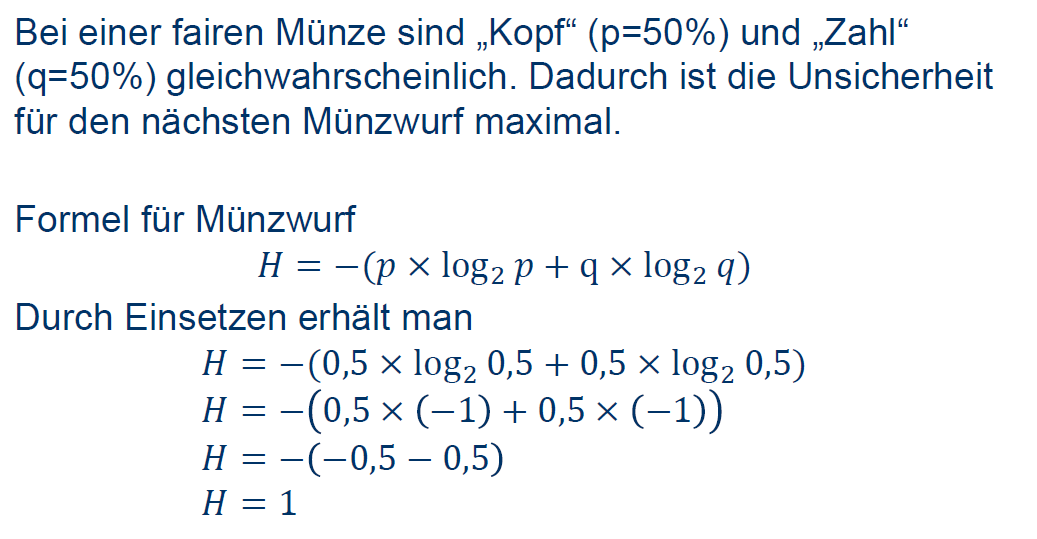
\includegraphics{img/Bsp fairer Munzwurf.png}
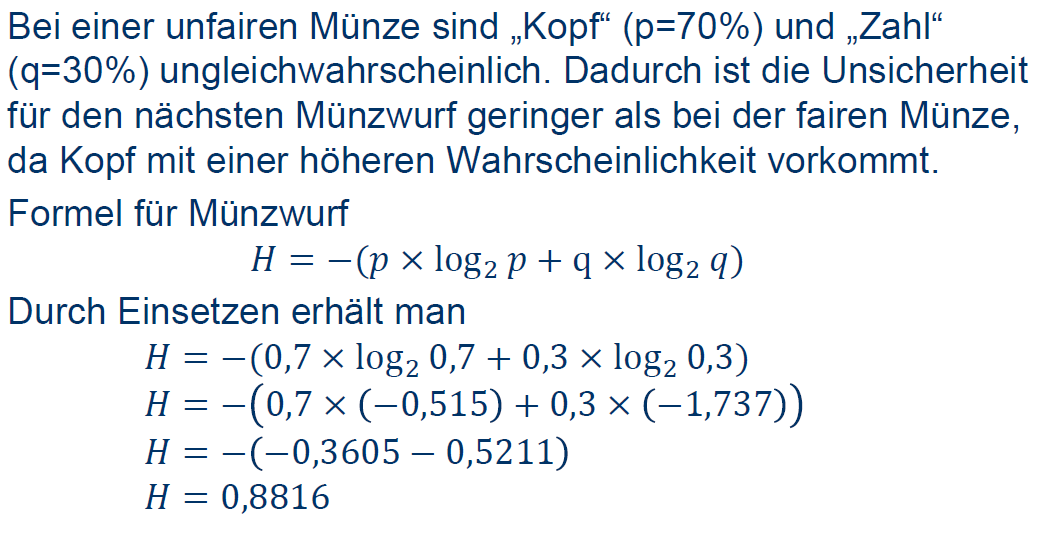
\includegraphics{img/Bsp unfairer Munzwurf.png}

Eine Information kann viele Eigenschaften haben, die ihren Wert
beeinflussen. \textbf{Aktualität} bezieht sich auf die Frage, wie weit
in der Zeit der Zustand zurückliegt, auf den sich die Information
bezieht. \textbf{Korrektheit} bezieht sich auf den Wahrheitsgehalt der
Information. \textbf{Genauigkeit} bezieht sich auf die Präzision der
Information. Der \textbf{Aggregationsgrad} von Informationen sagt etwas
über die Bezugsobjekte oder -ereignisse aus. Die \textbf{Präsentation}
einer Information ist ebenso wichtig, da die volle Ausschöpfung des
Informationswerts davon abhängt, dass der Empfänger die Information
vollständig aufnimmt. Die \textbf{Kosten} einer Information sind
insbesondere bei ex ante (von Anfang an) Betrachtungen wichtig, wenn
über die Beschaffung der Information entschieden werden muss.

\emph{Folgend sind einige Informationsattribute und ihre möglichen
Ausprägungen dargestellt.}

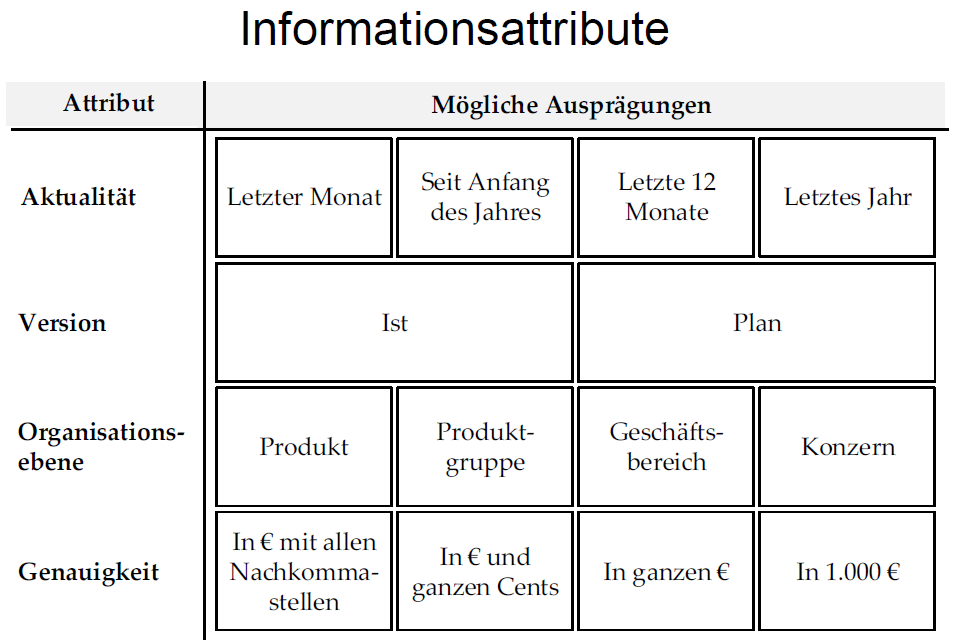
\includegraphics{img/Informationsattribute.png}

\begin{itemize}
\tightlist
\item
  \textbf{Problemlösungsprozess}
\end{itemize}

Generell werden Informationen benötigt, um eine Entscheidung zu treffen
oder eine Kontrolle vorzunehmen. Informationen sind als Rohstoff für
Entscheidungs- und Kontrollprozesse zu betrachten.

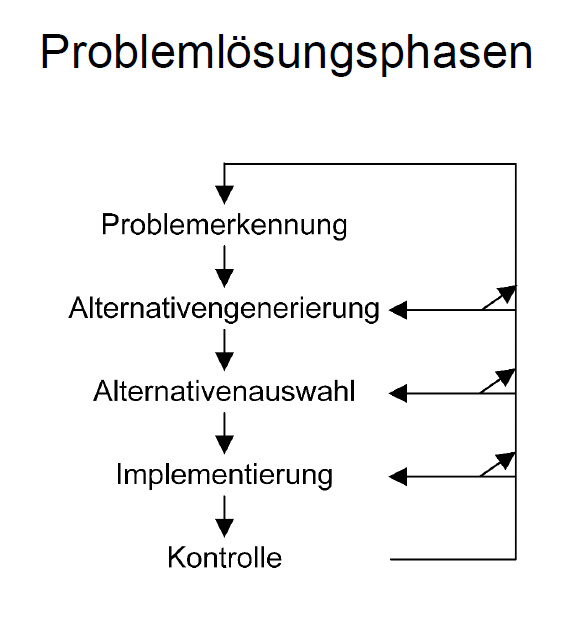
\includegraphics{img/problophasen.png}
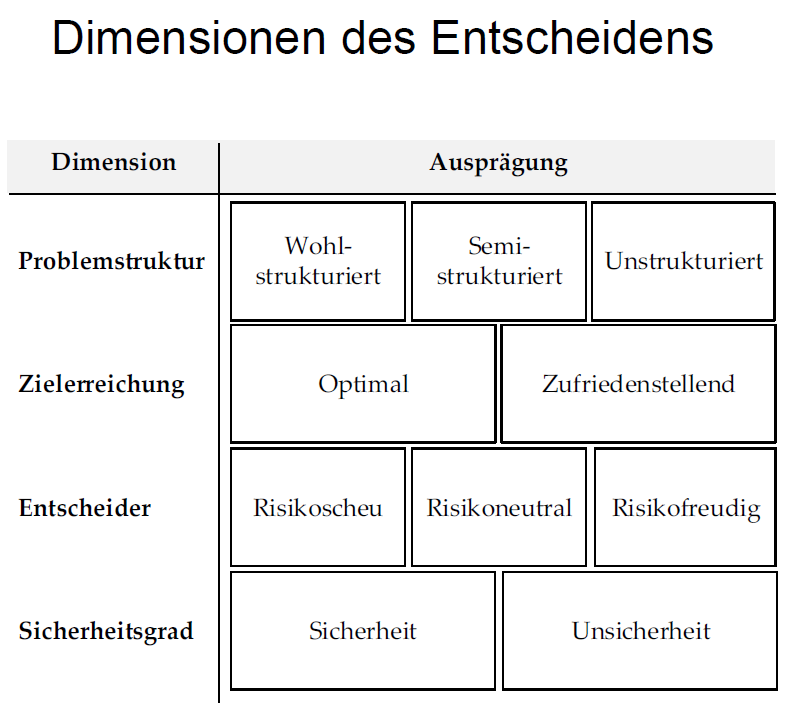
\includegraphics{img/dimensionentscheiden.png}

Wenn eine Entscheidungsträger hinsichtlich eines Problems zu jeder der
Phasen ein geeignetes Vorgehen kennt, ist das Problem für ihn
\textbf{wohlstrukturiert}. Im anderen Extremfall, wenn zu keiner der
Phasen ein geeignetes Vorgehen bekannt ist, wird das Problem als
\textbf{unstrukturiert} bezeichnet. Dazwischen sind die
\textbf{semistrukturiertem} Probleme. Hier sind Lösungsansätze zwar für
einige der Phasen, aber nicht für alle Phasen bekannt.

In der Entscheidungstheorie wird zwischen Entscheidungen unter
\textbf{Sicherheit} und unter \textbf{Unsicherheit} unterschieden. Im
ersten Fall liegen sämtliche Prognosedaten über die
Entscheidungskonsequenzen der zu beurteilenden Alternativen in
einwertiger Form vor. Bei Entscheidungen unter Unsicherheit werden die
Konsequenzen mehrwertig notiert. Mehrwertigkeit liegt z.B. dann vor,
wenn Vorhersagen für verschiedene Szenarien getroffen werden.

Die Persönlichkeit des Entscheidungsträgers drückt sich auch in seiner
Risikoeinstellung aus. Diese kann aufgrund des
\textbf{Nutzenerwartungswerts} bei einem zufallsbedingten Ereignis
bestimmt werden:


\includegraphics{img/nutzerwert.png}

wobei p(i) die Eintrittswahrscheinlichkeit des Ereignisses x(i) ist und
N(x(i)) der Nutzen, den der Entscheidungsträger dem Eintreten des
Ereignisses x(i) beimisst. Der Nutzenerwartungswert kann mit einem
sicheren Wert verglichen werden, dem sog. \emph{Sicherheitsäquivalent},
den der Entscheider auswählt bzw. bei einem Glücksspiel als Spieleinsatz
akzeptiert. Wenn die beiden Werte gleich sind, dann wird der Entscheider
als \textbf{risikoneutral} bezeichnet. Wenn sich der Entscheider für ein
ihm angbotenes Sicherheitsäquivalent entscheidet, das kleiner als der
Nutzenerwartungswert ist, dann ist der Entscheider \textbf{risikoscheu};
wenn er sich für den höheren Nutzenerwartungswert entscheidet, ist er
\textbf{risikofreudig}. Im letzteren Fall zieht er die Chance auf den
Erhalt eines größeren Nutzens einem sicheren, kleineren Nutzen vor.

\begin{itemize}
\tightlist
\item
  \textbf{Wert von Informationen:}
\end{itemize}

\begin{enumerate}
\def\labelenumi{\arabic{enumi}.}
\tightlist
\item
  \textbf{Subjektiver Ansatz}:
\end{enumerate}

Man befragt den Informationsbenutzer, wie viel ihm die Information wert
ist. Dieser Ansatz wird insbesondere dann gewählt, wenn es sich um
unstrukturierte Probleme unter Unsicherheit handelt. Seine Stärke, die
nachfragebezogene Wertbestimmung, ist gleichzeitig auch seine Schwäche,
nämlich die mangelnde Nachprüfbarkeit der Korrektheit. Es ist möglich,
den Grad der Subjektivität zu verringern, indem mehrere Benutzer in
einer Organisation befragt und die Antworten in geeigneter Weise
zusammengefasst werden.

\begin{enumerate}
\def\labelenumi{\arabic{enumi}.}
\setcounter{enumi}{1}
\tightlist
\item
  \textbf{Objecktiver Ansatz}:
\end{enumerate}

Ein objecktiver Ansatz ist die Ermittlung des beobachtbaren Werts von
Informationen. Dabei wird das Ergebnis eines Entscheidungsprozesses mit
und ohne eine bestimmte Information betrachtet. Die Ergebnisdifferenz
entspricht dem Informationswert, wenn man all anderen Einfüsse konstant
halten kann (in dieser Bedingung verbirgt sich die Schwierigkeit des
Ansatzes). Der Vorteil besteht darin, dass er die tatsächlich erreichten
Ergebnisse berücksichtigt und damit die Fähigkeiten und
Zielerreichungsbedürfnisse der Entscheidungsträger. Ein Nachteil ist,
dass der Wert nur ex post ermittelt werden kann, wenn man die
Information schon erworben hat. Die Wertermittlung kann jedoch auch für
diesen Fall sinnvoll sein, um für den Wiederholungsfall zu lernen.

\begin{enumerate}
\def\labelenumi{\arabic{enumi}.}
\setcounter{enumi}{2}
\tightlist
\item
  \textbf{Normativer Ansatz}:
\end{enumerate}

Ein normativer Ansatz, der auch ex ante angewendet werden kann, ist die
Bestimmung des normativen Werts der Information. Hier wird der
Informationswert durch die Differenz des erwarteten Gewinns mit der
betreffenden Information und dem erwarteten Gewinn ohne die Information
gemessen. Der Nachteil dieses Verfahrens ist, dass die Güte der
Information nicht leicht bestimmbar und nachprüfbar ist.

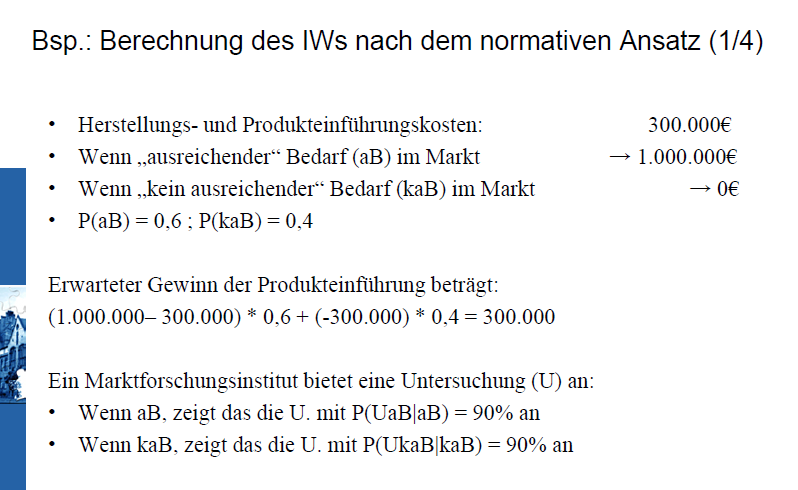
\includegraphics{img/Nansatz1.png} 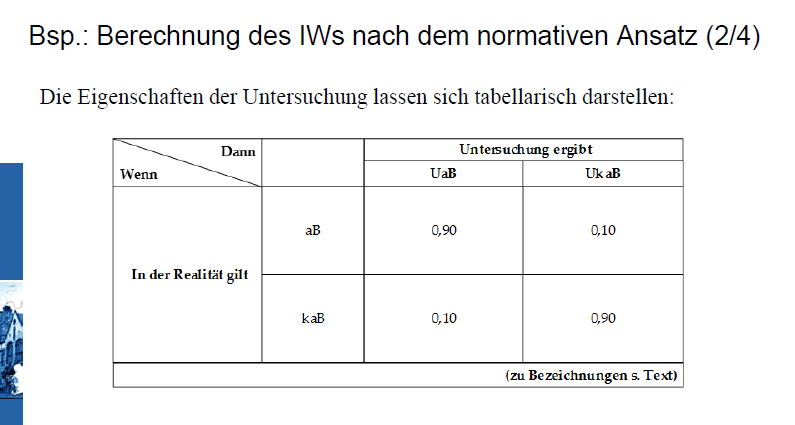
\includegraphics{img/Nansatz2.png}
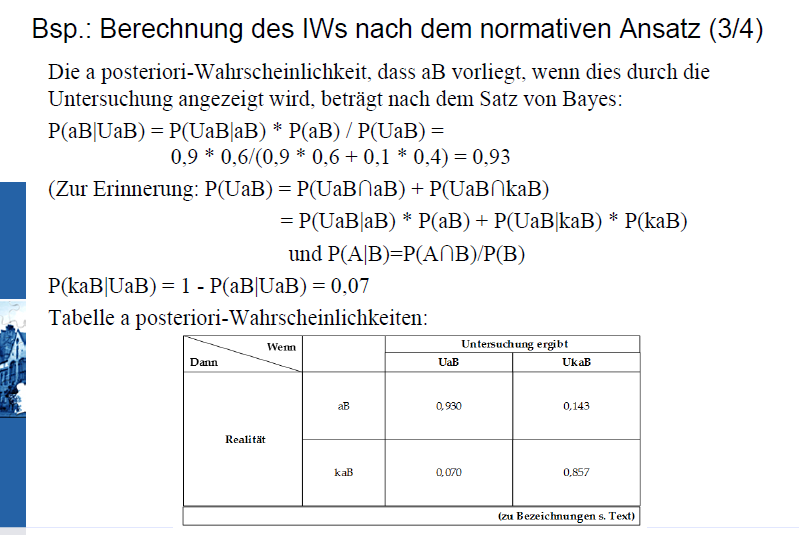
\includegraphics{img/Nansatz3.png} 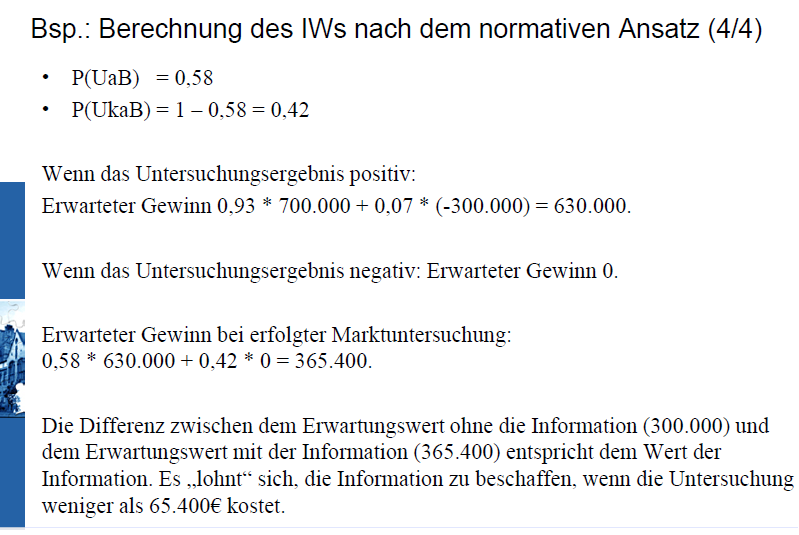
\includegraphics{img/Nansatz4.png}

In der Praxis wird der Wert einer Information oft nicht im Kontext von
``mit'' oder ``ohne'' Information ermittelt, sondern es werden
Informationen mit unterschiedlichen Ausprägungen eines oder mehrerer
Attribute betrachtet, um eine zufriedenstellende Konstellation
auszuwählen.

Abschließend ist festzuhalten, dass das Ergebnis eines
Entscheidungsprozesses, in den Informationen eingeflossen sind, wiederum
eine Information darstellt.

\begin{itemize}
\tightlist
\item
  \textbf{System}
\end{itemize}

Ein \textbf{System} besteht aus einer Menge von miteinander verknüpften
Elementen, die sich insgesamt von ihrer Umgebung abgrenzen lassen.
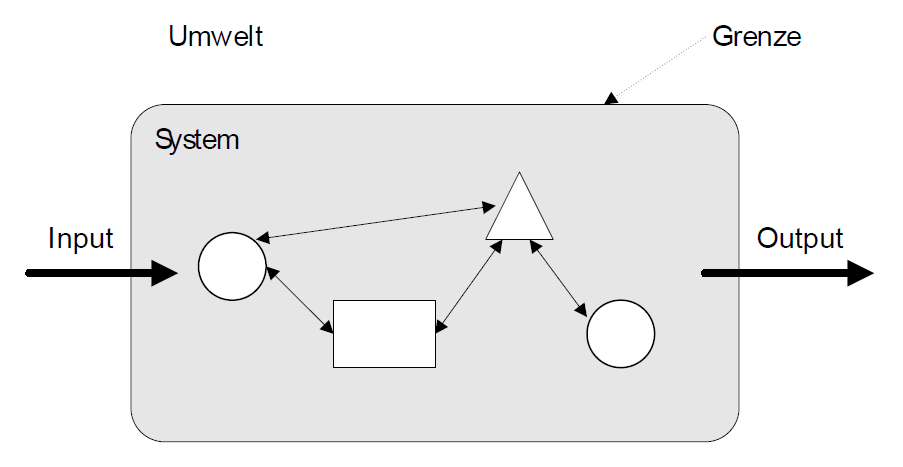
\includegraphics{img/systemdefi.png}

Diese Grafik enthält zusätzlich Eingaben und Ausgaben, die das System
mit der Umwelt austauscht. Diese sind in der Definition nicht enthalten,
weil es geschlossene Systeme gibt, die mit ihrer Umwelt nichts
austauschen.

Die Ermittlung der Grenzen eines Systems und der Beziehungen zwischen
seinen Elementen können schwierig sein. Wenn man an den Elementen und
ihren Beziehungen nicht interessiert ist, sondern nur an der Verwendung
eines Systems, dann bezeichnet man das System als eine ``Blackbox''. Es
reicht oft aus zu Wissen, welche Inputs zu welchen Outputs führen, um
ein System zu nutzen. Ein Element eines Systems kann ebenfalls ein
System sein (Subsystem). 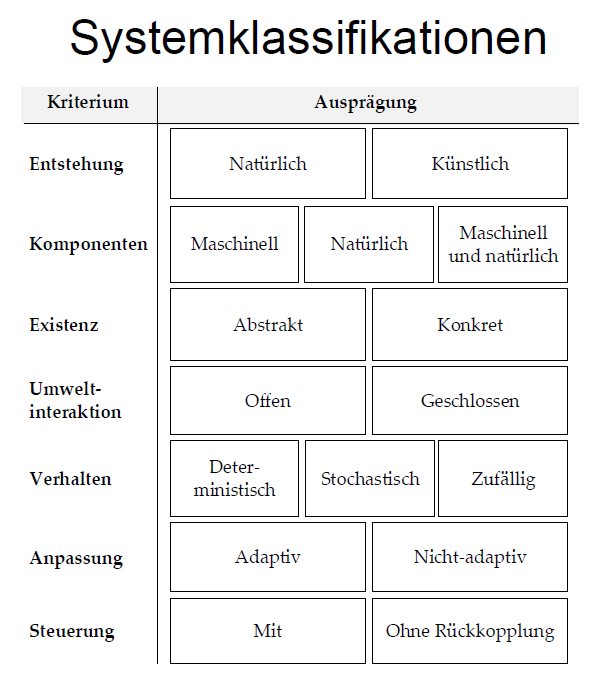
\includegraphics{img/systemcl.png}

Ein System, dessen Verhalten exakt vorraussagbar ist, wird als
\textbf{deterministisch} bezeichnet. Wenn das Verhalten (nur) einer
Komponente eines Systems einer Wahrscheinlichkeitsverteilung folgt (z.B.
bezüglich ihres Ausfalls), so ist das gesamte System
\textbf{stochastisch}. Wenn ein Beobachter nicht einmal
Wahrscheinlichkeiten für das Verhalten eines Systems kennt, verhält sich
das System für ihn \textbf{zufällig}.

In vielen Organisationen werden die realisierten Ergebnisse regelmäßig
mit angestrebten Zielen verglichen. Wenn die Übereinstimmung als nicht
zufriedenstellend angesehen wird, werden die Systemeingaben und/oder das
interne Systemverhalten geändert. Man spricht hier von
\textbf{Rückkopplung}.

\begin{itemize}
\tightlist
\item
  \textbf{Modell}
\end{itemize}

Ein \textbf{Modell} ist das Ergebnis eines Konstruktionsprozesses, das
die Wahrnehmung von Inhalten eines ausgewählten Gegenstands
zweckorientiert repräsentiert. In Modellen werden die für nicht relevant
angesehenen Eigenschaften eines Systems weggelassen. Mit einem Modell
kan somit einfacher experimentiert werden, um das zu analysierende
System bzw. das Original besser verstehen bzw. steuern zu können, ohne
dieses selbst zu beeinflussen. Die Qualität des Modells ist daran zu
beurteilen, inwiefern die Repräsentation geeignet ist, die Zwecke des
Modellnutzers zu erfüllen.

\texttt{!{[}modellcl{]}(img/modellcl.png)}

\begin{figure}
\centerline{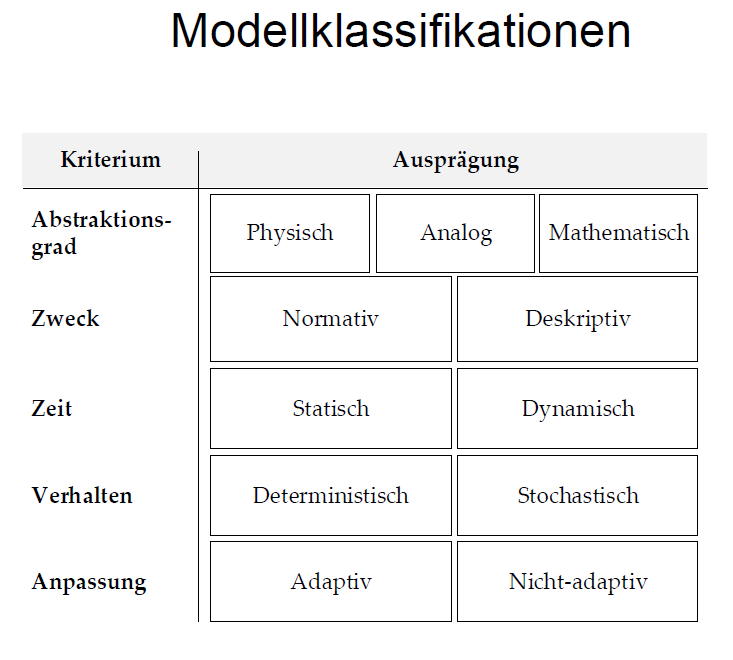
\includegraphics[width=0.8\textwidth]{img/modellcl.png}}
\caption{fake and gay}
\end{figure}

Der Zweck eines Modells kann sein, ein System zu beschreiben
(\textbf{deskriptiv}) oder Handlungen zu empfehlen (\textbf{normativ}).
Wenn das Modell Größen beinhaltet, die sich auf mehr als einen Zeitpunkt
beziehen, wird von einem \textbf{dynamischen} (also
\textbf{mehrperiodigen}) Modell gesprochen. In \textbf{statischen}
(\textbf{einperiodigen}) Modellen beziehen sich alle Variablen auf den
gleichen Zeitpunkt bzw. Zeitraum.

\begin{itemize}
\tightlist
\item
  \textbf{Modelle von Unternehmungen}
\end{itemize}

Aus der Sicht der Systemtheorie enthalten Organisationen i.d.R.
maschinelle und natürliche Komponenten und sind meistens offene,
adaptive Systeme mit Rückkopplung. Da eine Organisation viele
Komponenten enthält, ist zwecks Erreichung der Organisationsziele eine
Koordination dieser Komponenten notwendig. Diese Koordination wird durch
eine Aufbausorganisation, die Aufgaben, Aufgabenträger und ihre formalen
Beziehungen untereinander festgelegt, und durch eine Ablauforganisation,
die Arbeitsabläufe bestimmt, unterstützt.

In vielen Organisationen herrscht hierarchische Koordination mit einer
oder mehreren Leitungsebenen vor. Die Leitungs- oder
Managementfunktionen werden oft in drei Ebenen unterteilt. Die Manager
einer Ebene haben Mitarbeiterverantwortung für die unteren Ebenen. In
der näschten Abbildung sind die Leitungsebenen um die Ausführungebenen
ergänzt, damit die gesamte Unternehmung in dem Modell repräsentiert
wird. Die Linien die die Pyramide vertikal unterteilen, trennen die
verschiedenen funktionalen Bereiche, wie etwa Beschaffung, Produktion
oder Vertrieb, voneinander ab. 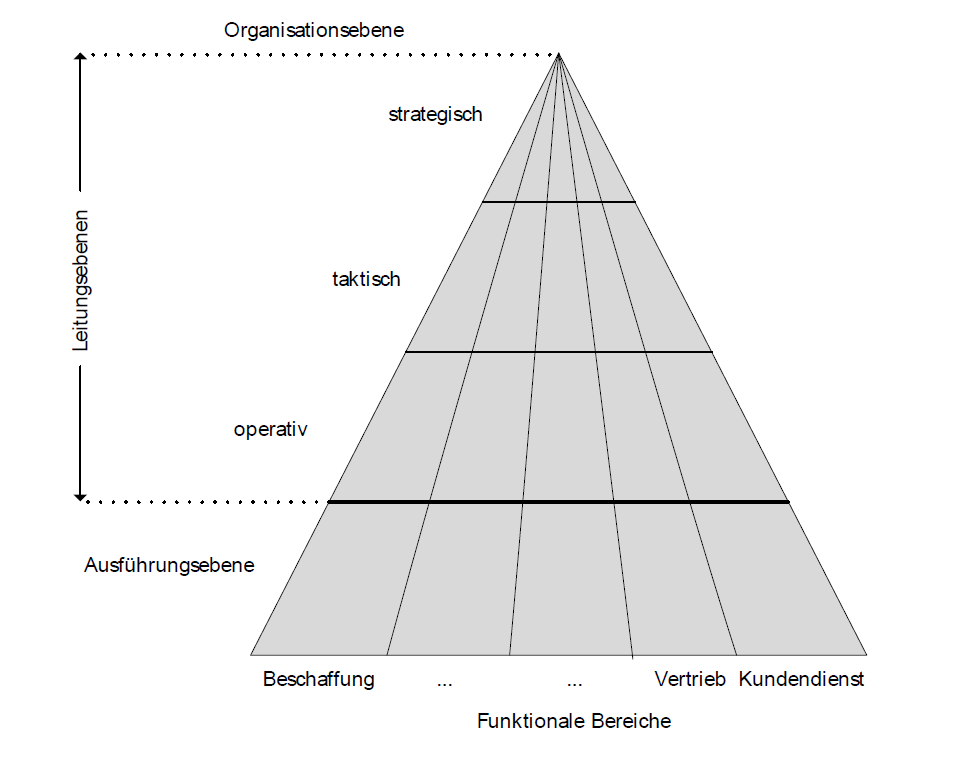
\includegraphics{img/orgaeben.png}

Die unterschiedlichen Aufgaben der Manager auf den drei Ebenen führen zu
unterschiedlichen Informationsbedürfnissen. Diese werden in der nächsten
Tabelle dargestellt. Dabei sind die Einträge so zu interpretieren, dass
z.B. bezüglich der Herkunft der Informationen die operative Ebene
vorwiegend interne Informationen benötigt, die strategische Ebene
vorwiegend externe Informationen und die taktische Ebene dazwischen
liegt. 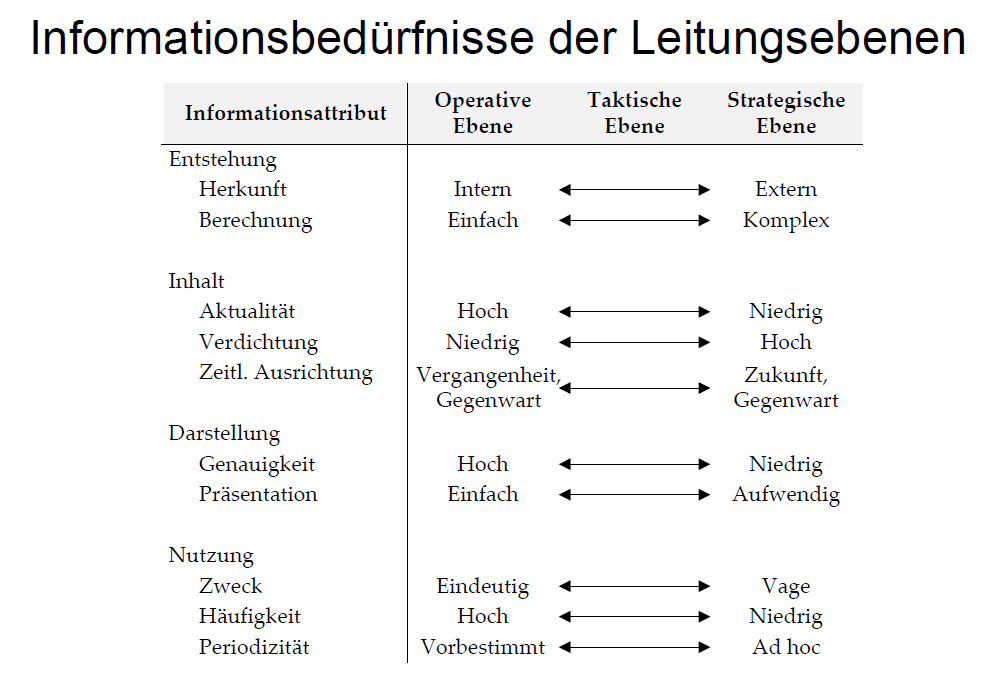
\includegraphics{img/infobedarf.png}

Heute wird versucht, ``flache'' Organisationen mit möglichst wenig
Personal, das nur überwacht und informiert, zu entwickeln. Die
Entwicklung solcher Organisationen unterstützen IS erheblich. Die vorher
genannten planerischen Aufgaben existieren trotz Verflachung der
Organisation weiter.

Das Handeln einer Unternehmung beeinflussen nicht nur ihre Mitarbeiter
und ihre direkten Geschäftspartner, sondern eine Vielzahl an
Interessengruppen. Diese Gruppen werden gleichzeitig durch das Handeln
der Unternehmung beeinflusst. Das gezeigte Modell einer Unternehmung als
Führungssicht versucht, die Komplexität ihrer Beziehungen durch sechs
Grundkategorien einzufangen:

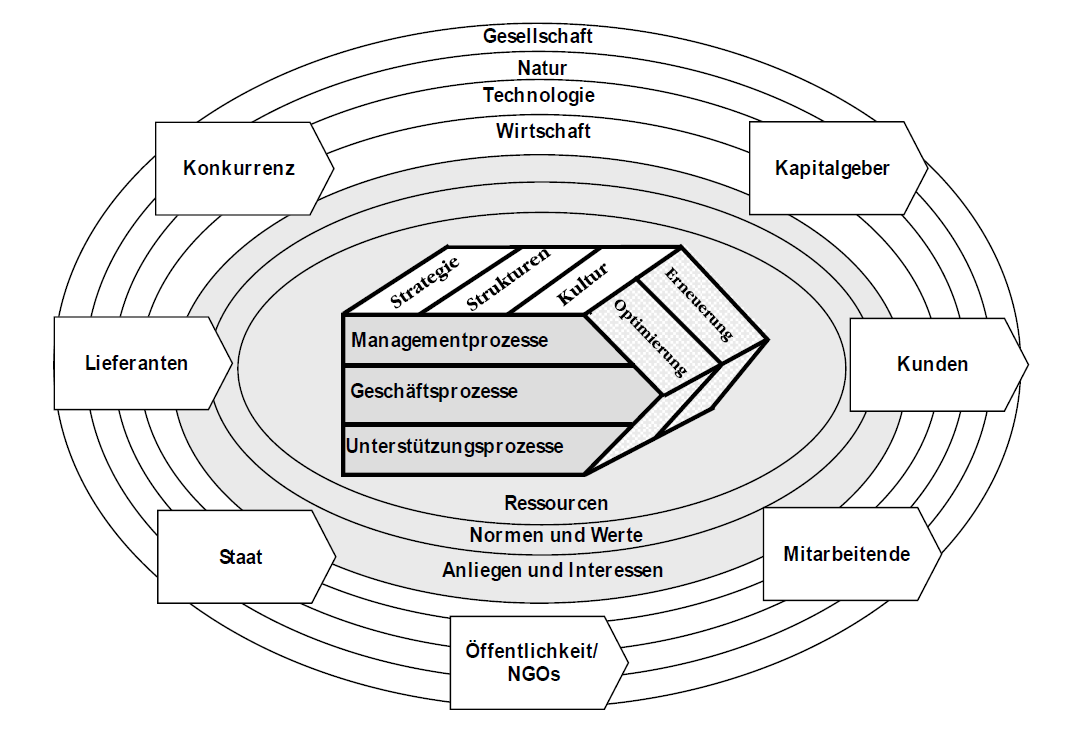
\includegraphics{img/manamodell.png}

\begin{enumerate}
\def\labelenumi{\arabic{enumi}.}
\tightlist
\item
  \emph{Umweltsphären} (Gesellschaft, Natur, Technologie, Wirtschaft)
  sind Rahmenbedingungen, die ständig auf Veränderungen beobachtet
  werden sollten und teilweise beeinflusst werden können.
\item
  \emph{Anspruchsgruppen} (Kapitalgeber, Kunden, Mitarbeitende, usw.)
  stehen in beabsichtigten Austauschprozessen mit der Unternehmung oder
  werden von ihren Handlungen mehr oder weniger zufällig betroffen (z.B
  durch Umweltbelastung oder Sponsoring).
\item
  \emph{Interaktionsthemen} (Ressourcen, Normen und Werte, Anliegen und
  Interessen) repräsentieren den Austausch zwischen der Unternehmung und
  den Anspruchsgruppen, der materieller (Güter) oder immaterieller (z.B.
  Rechte, Anliegen oder Normen) Art sein kann.
\item
  \emph{Ordnungsmomente} (Strategie, Strukturen, Kultur) stellen das
  interne Rahmenwerk der Unternehmung dar, indem sie Ziele und
  formale/informale Kommunikationsstrukturen bestimmen.
\item
  \emph{Prozesse} bilden die sachlichen und zeitlichen Bedingungen und
  Abfolgen der Leistungserbringung ab.
\item
  \emph{Entwicklungsmodi} (schattierte Seitenfläche des Polyeders)
  zeigen Möglichkeiten der Weiterentwicklung auf, die aus der
  Verbesserung bestehender Prozesse (Optimierung) oder aus der
  Transformation unter Ausnutzung von Innovationen (Erneuerung)
  bestehen.
\end{enumerate}


\end{document}
